\documentclass[../SimBALink.tex]{subfiles}
\begin{document}

\section{Environment} This system models the environment of the motorcycle is riding in.

Force directions are defined as longitudinal(long), lateral(lat), and normal(n). Longitudinal is along the direction of the motorcycle (when moving straight). Lateral is orthogonal to Longitudinal axis. Normal 3-D orthogonal to lateral and longitudinal, in general the axis to the road on no incline.

\subsection{Inputs and outputs}
	\subsubsection{Inputs}
	\begin{tabular}{ l | l | l  }
		Input					&	Symbol		&	Unit		\\	\hline
		Distance Travel			&	$d$			&	m
	\end{tabular}
	
	\subsubsection{Outputs}
	\begin{tabular}{ l | l | l  }
		Output								&	Symbol		&	Unit		\\	\hline
		Environment Forces on Tire[3]		&	$F_t$		&	N[3] \\
		Road Gradient						&	$\theta_r$	&	rad \\
		Ambient Temperature					&	$T_{amb}$	&  K \\
		Air Pressure						&	$P$  		& Pa \\
		Air Density 						&	$\rho$		& $kg/m^3$ \\
		Corner Radius 						&	$R_c$		& $m$
	\end{tabular}

\subsubsection{Background, rationale, modeling strategy}
The Environment only models air density, air temperature, and road gradient.
	\begin{gather}
		\theta_r  = \arctan\left(\frac{\frac{d}{dt} h(d)}{\frac{d}{dt} d}\right) \\
		T_{amb} = T_0 - L h(d) \\
		P = P_0 \left( 1 - \frac{L h(d)}{T_0} \right)^{\frac{gM}{RL}}\\
		\rho = \frac{PM}{1000RT}  
\end{gather}
\subsubsection{Parameters}
	\begin{tabular}{ l | l | l  }
		Parameter					&	Symbol		&	Unit		\\	\hline
		Temperature Lapse		&	$L$			&	 $K/m$ \\
		Initial Pressure 		&  $P_0$		&	$Pa$ \\
		Initial Temperature		&  $T_0$		&	K \\
		Gravity 				&  $g$			&  $m/s^2$ \\
		Molar mass of Dry Air	& $M$			&  kg/mol \\
		Ideal Gas Constant 		& $R$			& $\frac{J}{mol * K}$
	\end{tabular}
	
	\subsubsection{Look up Table}
	$h(d)$ \\
	\begin{tabular}{ l | l | l | l }
		Type				& Description		&	Symbol		&	Unit		\\	\hline
		Input 				& Distance Travel	&	$d$  		& m		\\
		Output 				& height 			&	n/a			&  m
	\end{tabular} \\
		$R_c(d)$ \\
	\begin{tabular}{ l | l | l | l }
		Type				& Description		&	Symbol		&	Unit		\\	\hline
		Input 				& Distance Travel	&	$d$  		& m		\\
		Output 				& Corner Radius 	&	n/a			&  m
	\end{tabular} \\
\subsubsection{Assumptions}
\begin{itemize}
  \item The air is dry 
  \item Temperature lapse rate right is correct (no inversion)
\end{itemize}

\section{Validation}

To validate the road gradient the Isle of Man altitude map was supplied to the model and the road gradient was plotted. To validate air density data from Colorado was compared to a simulated data.

\begin{figure}[H]
\center
 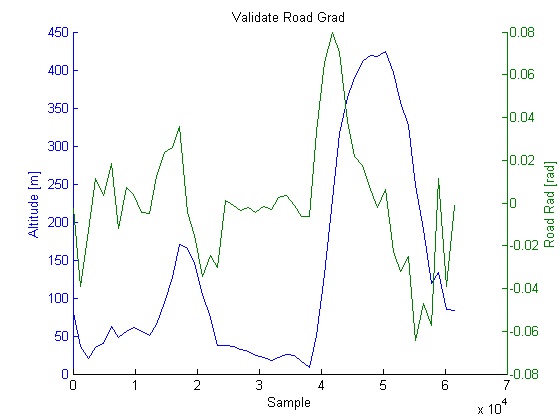
\includegraphics[scale=1]{env_val_grad}
 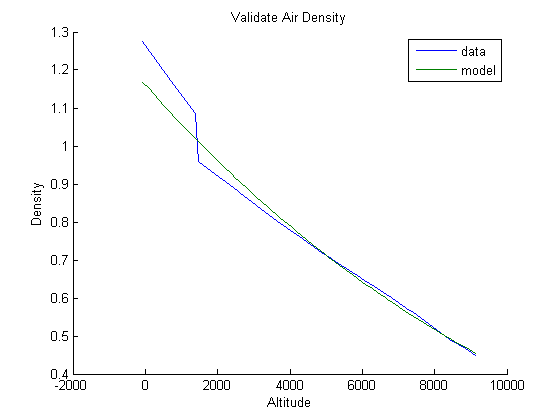
\includegraphics[scale=1]{env_val_rho}
  \caption{Environment Validation}
\end{figure}


\end{document}